Baseret på den viden der er blevet indsamlet, laves der er et proof of concept til søvndelen af projektet.
Denne implementering er beskrevet herunder.
Grunden til at der kun laves et proof of concept og ikke et fuldstændigt færdigt system er, at der ikke er nok tid til at gøre det helt færdigt. 
Ydermere, vil et helt færdigt system påkræve testning hos målgruppen, og dette er der ikke er tid nok til at udføre. 

Denne sektion om proof of concept beskriver valg af nødvendig sensor data, hvordan søvnestimering udføres på data, og hvordan søvnestimeringerne for de forskellige sensorer kombineres og hvordan denne estimeringen skal aggregeres til individuelle perioder af søvn.

% Manglende resourcer
% Time constraints.
% Ingen test mulig(Kræver tilladelser, og system ikke færdig)

Som et proof of concept er der blevet valgt at implementere en enkelt metode til at afgøre hvorvidt man sover eller ej.
Metoden er baseret på redskaberne beskrevet i \cref{sec:redskaber}, hvor der som start til dataindsamling ses på amplitude og acceleration.
Grunden til at vi starter med disse to datakilder er fordi \citet{6563918} erfarede, at det er de langt væsentligste datakilder, hvilket også er beskrevet i \cref{sec:BES}.

Disse to datakilder kombineres til en enkelt model, der skal kunne afgøre hvorvidt man sover eller ej.
Med mere tid vil de andre nævnte datakilder også blive fokuseret på.

For at have en regelmæssig måde at indsamle data, der ligger til grund for implementeringen af det efterfølgende søvnestimeringsmetode, er det nødvendigt at have forsøgsopstillingen beskrevet, hvorfor denne følger herefter.
\subsection{Forsøgsopstilling}
%Disposition:
%Billede af opstilling
%Bare tage med hjem og sove
%Flere forsøg og systematisk tilgang kunne være brugt og skulle gøres hvis det ikke bare var proof of concept.
For at forsøget fortages på samme måde hver gang, så det indsamlede data er sammenligneligt, valgte vi at lave en forsøgsopstilling.
\begin{figure}[h]
	\centering
	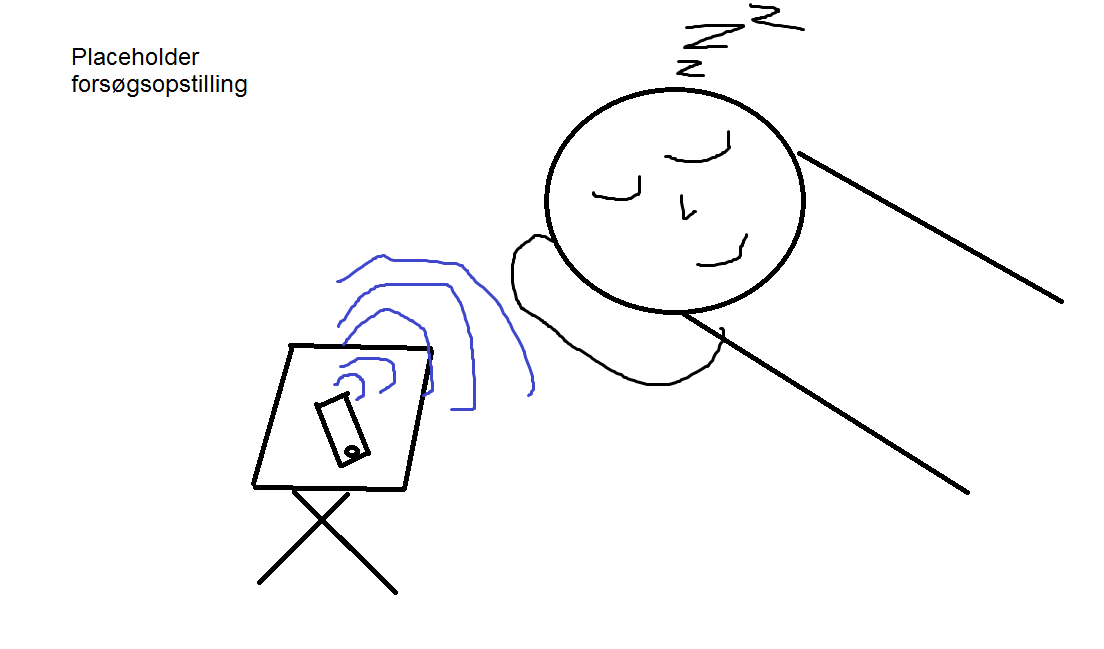
\includegraphics[scale=0.5,trim = 0cm 0cm 5cm 10cm, clip]{forsoegsopstilling}
	\caption{Forsøgsopstilling. Sovende person med telefonen på natbordet.}
	\label{fig:forsoegopstillings}
\end{figure}

Forsøgsopstillingen kan ses i \cref{fig:forsoegopstillings} der illustrerer hvordan telefonen ligger på natbordet og indsamler data.
Idéen er at det eneste krav til indsamlingen er, at den skal ligge på et bord i soveværelset når der soves, ellers står det en frit om man går med telefonen i lommen, lægger den på skrivebordet eller andet. 
Dette valg er foretaget i henhold til vores kriterie om at udvikle et system der kan måle søvn uden at forstyrre.

Indsamlingen af data foregik ved at vi installerede de fornødne moduler på egen telefon, Tog telefonen med hjem, så data fra en eller flere dage kunne indsamles.
Vi loggede fra vi gik i seng til vi stod op, hvilket skulle bruges til at afgøre nøjagtigheden af vores estimat.

Til at validere vores model har vi foreslået krydsvalidering beskrevet i \cref{sec:redskaber}, hvilket også bør gøres med mere tid, men da dette er et proof of concept er den nuværende opstilling tilfredsstillende.
Ved videre arbejde bør en mere systematisk tilgang med den nævnte krydsvalidering benyttes, hvilket er beskrevet videre i \cref{sec:verisoevn}.

\subsection{Sensor Data}
For at have en bedre indsigt i hvordan vi kan bruge accelerations- og amplitude-data blev disse plottet over en dag inklusiv søvn.
Dette kan ses i \cref{fig:accplot} og \cref{fig:amplplot}.

\begin{figure}[h]
	\centering
	%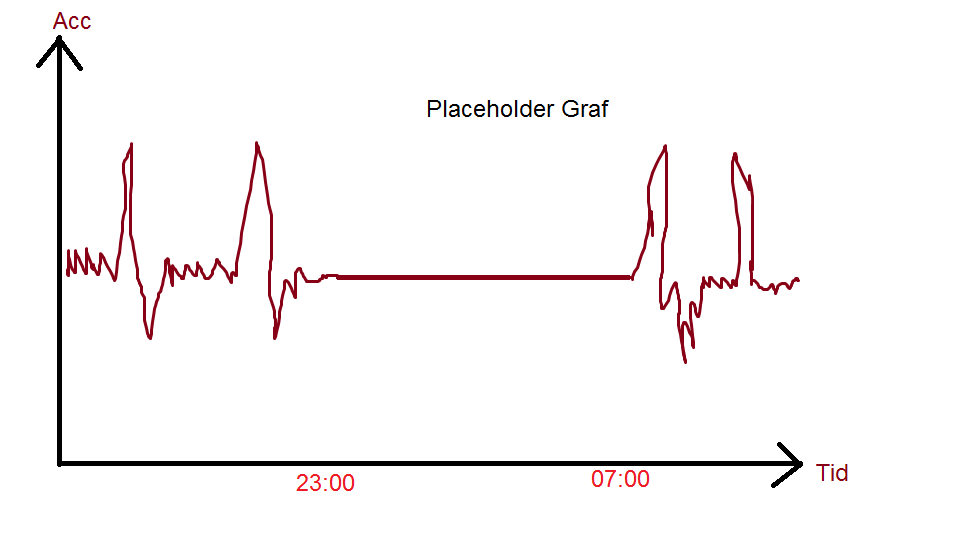
\includegraphics[scale=0.5]{acc-placeholder}
	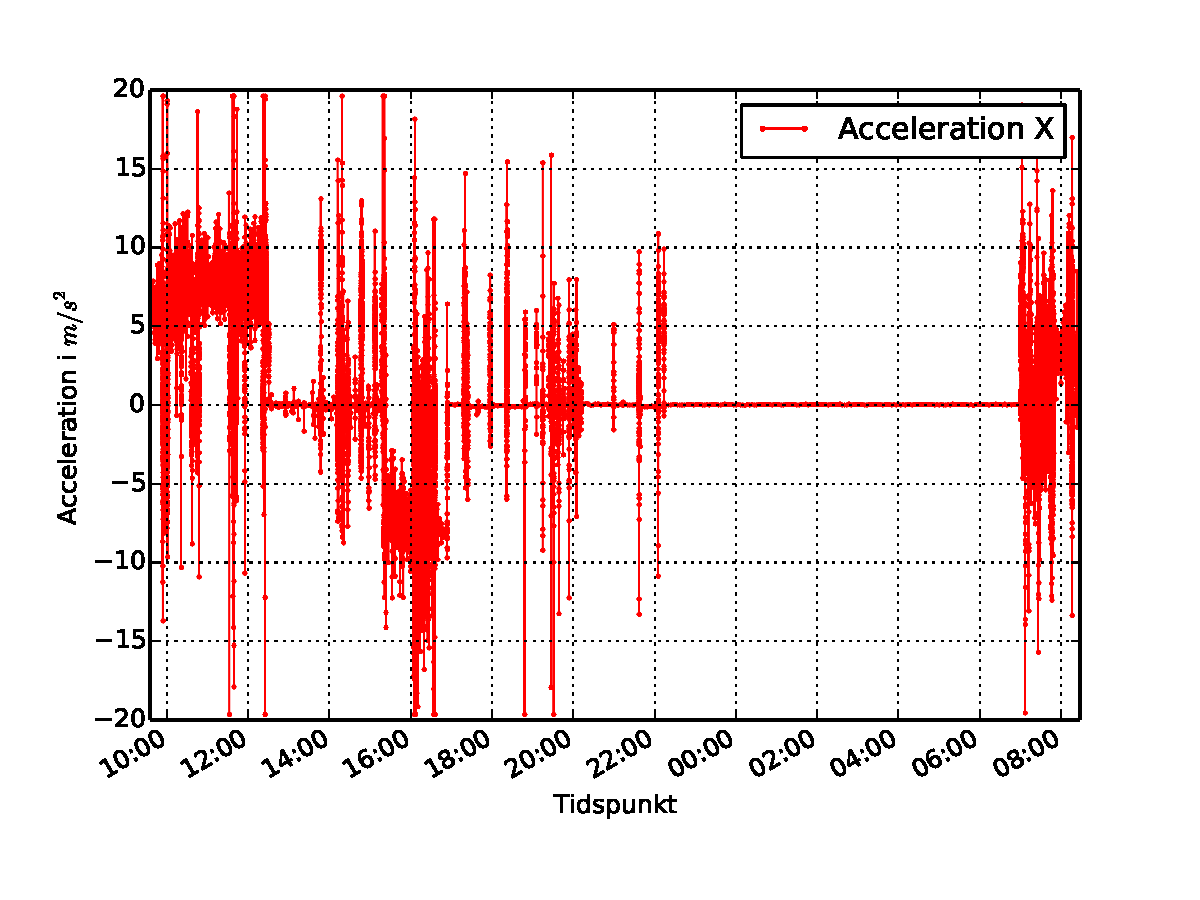
\includegraphics[scale=0.75]{acceleration-plot}
	\caption{Accelerationsplot, hvor der blev sovet fra ca. 22:00 til 07:00 næste dag.  Et punkt svarer til en måleværdi.}\label{fig:accplot}
\end{figure}

Ses der på accelerationsdata i \cref{fig:accplot} indikerer det tydeligt når telefonen har været i bevægelse og når telefonen ikke har været i bevægelse.
Dette skyldes at et accelerometer er god til at registrere bevægelse, da acceleration er ændring i hastighed.
Det viser sig at plottet fint indikerer når man er vågen, hvilket er forårsaget af at testpersonen har gået med sin telefon i lommen.
Dog kan man ved stilstand ikke vide sig sikker på om det er fordi man sover, eller blot fordi man har lagt sin telefon fra sig.

Ved stilstand i en længere periode, kan man estimere sandsynligheden for at denne stilstand er at brugeren sover. 
Derudover kan andre sensor inputs hjælpe til at klargøre denne tvivl, der ikke er begrænset til at man skal have telefonen i lommen.
Et eksempel på en sådan kilde er mikrofonen, som vi kan bruge til at måle maks amplitude.
At vi kun måler maks amplitude sikrer at personfølsomme oplysninger ikke indsamles, da man ikke kan genskabe en samtale, men blot har maks amplitude lagret for hvert sekund.

\begin{figure}[h]
	\centering
	%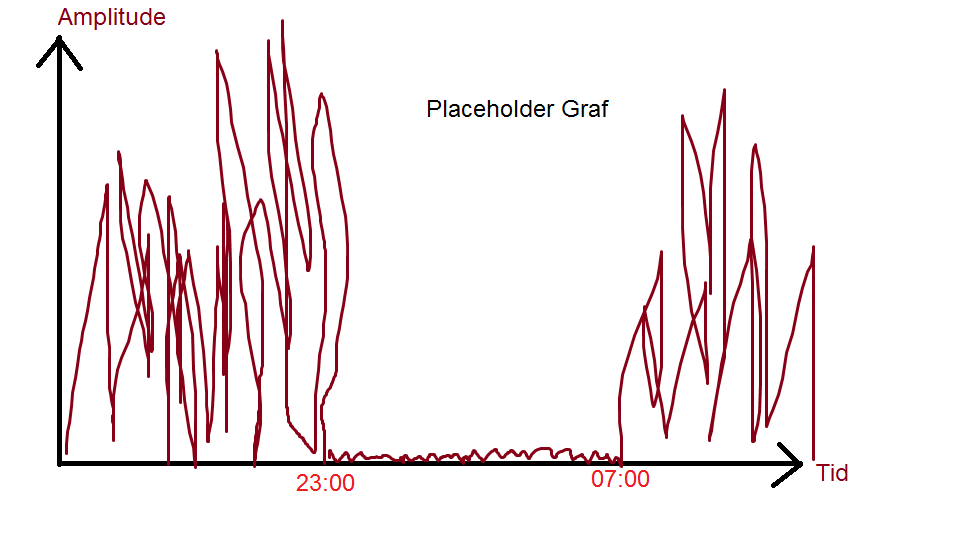
\includegraphics[scale=0.5]{ampl-placeholder}
	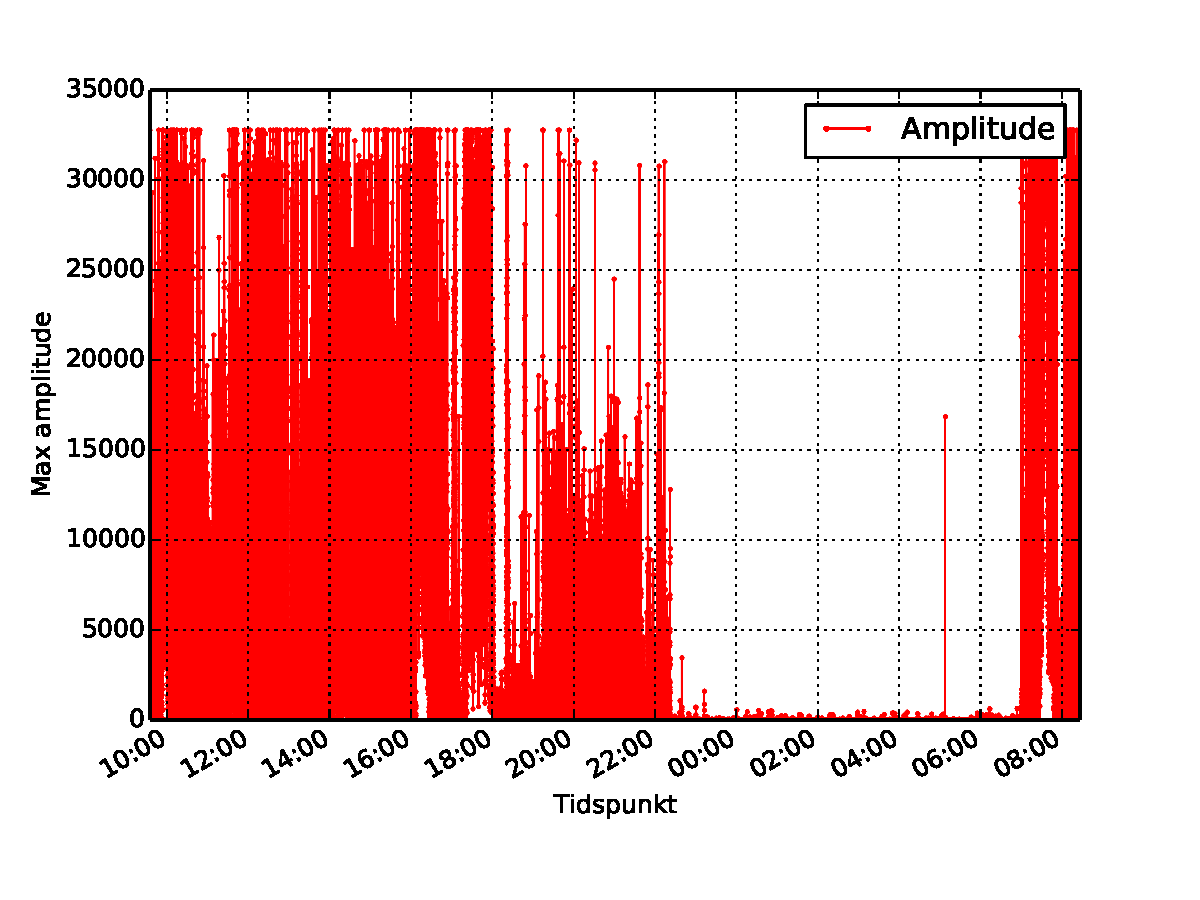
\includegraphics[scale=0.75]{amplitude-plot}
	\caption{Amplitudeplot, hvor der blev sovet fra ca. 22:00 til 07:00 næste dag. Et punkt svarer til en måleværdi.}\label{fig:amplplot}
\end{figure}

Idéen bag at bruge maks amplituden er at man larmer væsentligt mere når man er vågen end når man sover.
Dette passer fint med de loggede data der er plottet i \cref{fig:amplplot}.
Dog har denne antagelse også begrænsninger.
Eksempelvis kan det være at man er en stille person, snorker meget eller også kan personen bo i et meget larmende område.
Alligevel regner vi med at amplituden stadig kan bruges, da man så muligvis kan finde et mønster når man snorker til at styrke modellen, hvilket er diskuteret i \cref{section:snorken}.
Derudover, er det så et spørgsmål om hvor stor vægt man skal tillægge de enkelte sensorkilder, og er noget der bør trænes til det enkelte individ, for at opnå en model der passer til individets personlighed.
Hvordan dette gøres bør overvejes ved videreudvikling, men til dette proof of concept kan man som en start bruge fastsatte statiske vægte, hvilket er diskuteret i \cref{subsec:sensorvaegtsoevn}.

\subsection{Søvnestimerings model}
Ud fra observeret data etablerer vi nogle antagelser som vi går ud fra også holder til fremtidigt data.
Disse er at når man observerer en handling om det er acceleration eller amplitude, kan vi med stor sikkerhed sige at man ikke sover.
Modsat hænger sandsynligheden for at man sover sammen med længden af stilstand.

Dette får os til at lave en model der bygger på disse to antagelser, hvilket er gjort for at skabe jordforbindelse.
Dette betyder at vi udvikler en metode, for at bekræfte at det kan blive implementeret til en telefon med den valgte platform.
Som nævnt har vi ikke kunnet finde passende metoder, der er offentligt tilgængeligt, hvorfor vi bliver nødt til at udvikle vores egen metode.

Vores model går på en sliding window tilgang, hvor den centrale del er at registrere stilstand med acceleration og amplitude.
Konceptet om stilstand er taget fra \citet{6563918} angående Best Effort Sleep, og er hvilken model vores metode tager primært udgangspunkt i.
Toss 'N' Turns tilgang, hvor man ser på 10-minutters vinduer med data til at afgøre søvn eller ikke søvn er et alternativ.
Dette alternativ blev dog valgt fra i første omgang, som nævnt i \cref{subsec:summametoder}, da stilstandsbestemmelsen vurderedes mindre komplekst og egnede sig derfor bedre til en proof of concept løsning.
Med mere tid kunne Toss 'N' Turn tilgangen blive forsøgt implementeret.

\subsubsection{Stilstands Bestemmelse}
Som udgangspunkt for vores udkast til en søvnestimeringsmodel afgøres der hvornår der er stilstand.
Dette gøres forskelligt for acceleration og amplitude data, men tager udgangspunkt i det loggede data.
For at sikre at støj ikke påvirker resultatet kan der bruges forskellige strategier i brug. 
For eksempel hvis man ændrer drastisk på hvor ofte mikrofonen optager amplitude til f.eks. at optage hvert tiende sekund, vil dette resultere i færre datapunkter og hvis dette gøres indfanges der mindre støj.
Dog kan dette også håndteres på andre måder, for eksempel ved et glidende gennemsnit, nævnt i \cref{sec:redskaber}, udført på indsamlede data, men hvis man kan undgå at bearbejde data ved at indsamle mindre vil dette være en fordel.

Vi valgte at gøre det ved hjælp af et glidende gennemsnit fordi hvis man ændrer på hvor ofte sensorerne indsamler data, vil det muligvis have en påvirkning på andre moduler.
Derudover, hvis man skal indsamle færre datapunkter, er det vigtigt at vide hvor ofte man skal indsamle disse datapunkter for at undgå støj.
Dette vil dog kræve at man udfører eksperimenter for at finde ud af hvor ofte man skal indsamle datapunkter.
Dermed virkede det glidende gennemsnit til at være en simplere løsning til vores problem.

Hvis vi ser på \cref{fig:accplot}, der er et plot for accelerationsdata, kan vi se stilstand for punkterne mellem 22:00 og 07:00.
Øvelsen består i at have en metode der kan afgøre at disse punkter er i stilstand.
Dette gøres ved at for et givent punkt at se om de 5 tidligere målinger ikke afviger fra en given fastsat grænse fra punktet i betragtning i x, y og z aksen.
Pseudokode til at tjekke dette kan ses i \cref{lst:pseudoStationary}.

\begin{lstlisting}[caption={Pseudo kode for at tjekke om et punkt er i stilstand.}, label={lst:pseudoStationary}]
isStationary(accToConsider : AccelerationReading, previousPoints : Collection of AccelerationReadings) : boolean
   foreach acc in previousPoints
      if outOfThreshold(accToConsider, acc)
         return false
   return true
\end{lstlisting}

Hvis der ikke er en sådan afvigelse bestemmes det at punktet i betragtning er i stilstand.
Dette gøres for alle punkter og der afgøres for hvert af disse om de er i stilstand eller ej.
Ved at gøre det på denne måde er man robust overfor påvirkning af tyngdeaccelerationen, da denne vil måles konstant hvis telefonen ligger stille.

Ved at betragte amplituden \cref{fig:amplplot} kan her ses stilstand fra lidt over 22:00 til omkring 07:00 med lidt støj omkring klokken 05:00.
Som nævnt før bliver dette støj taklet af det glidende gennemsnit.
Derudover kan stilstandsbestemmelsen gøres på en måde der ligner den for accelerationen.
Der anvendes altså et sliding window, men i stedet for at se på om de 5 tidligere punkter afviger relativt i forhold til det givne punkt i betragtning ses der på om de alle ligger under en fastsat tærskel.
At se på 5 tidligere punkter er ikke en fastlagt værdi, men afhænger af indsamlingsfrekvensen, vi har for amplitude en indsamlingsfrekvens på en måling per sekund så tidshorisonten er på fem sekunder.
At kigge blot fem sekunder tilbage kan være op til debat, og ved videre arbejde er det en parameter man bør justere for at opnå en højere præcision.
Dog holder vi fast i at det er fornuftigt at kigge en tidsperiode tilbage i stedet for en fast mængde punkter.
Dette sikrer at algoritmen også er fremtidssikret med hensyn til dette, for ellers risikerer vi at nyt hardware har en højere indsamlingsfrekvens hvor at gå 5 punkter ikke ville fungere, men hvor en tidshorisont ville.
For at se indsamlingsfrekvensen på hardware se \cref{sec:metrikker}.

Dermed har vi nogle simple måder at afgøre stilstand på og kan bruges til vores søvnestimering.

\subsubsection{Søvnestimering}
Resultatet af stilstandsbestemmelsen er en række punkter der hver især er klassificeret som stilstand eller ikke stilstand.
Ud fra disse punkter kan der findes perioder med stilstand, og ud fra længden af hver af disse perioder tildeles punkterne en stigende sandsynlighed for søvn alt efter hvor langt fra starten af stilstandsperioden et af de givne punkter i perioden er.

Spørgsmålet går så på at finde en strategi der kan estimere søvnperioder. 
En mulig strategi ville være at finde starten og slutning af søvn og på den måde give en sandsynlighed for hvorvidt man sover.
En anden mulig strategi vil være at finde mønstre der indikere at man sover, altså at identificere en søvnperiode, og derudfra finde en start og slutning af ens søvn.

Vi har valgt at følge den første strategi fordi vores data tydeligt indikere hvornår man starter og stopper med at sove. 
Derudover, hvis man skal identificere en søvnperiode kræver det at man har en generel måde at genkende søvnperioder for mange forskellige personer.
Dette kan være problematisk, og derfor foretrækker vi den første strategi.

Spørgsmålet går så på hvorledes en funktion skal defineres for en sådan stigende sandsynlighed.
Det skal være en funktion der repræsenterer hvor sikker man er på søvn ud fra længden af stilstand eksempelvis målt i timer.
En sådan funktion bør være lært ud fra ens empiri, så man kan løse opgaven som et regressionsproblem.
Dette er et område der kan arbejdes videre med for at få en mere akkurat søvnestimeringsmetode og opfordres til at gøres med mere tid.

Dog for at få et udgangspunkt til diskussion af sådanne funktioner er der tre funktioner plottet i \cref{fig:trefunc}.
\begin{figure}[h]
	\centering
	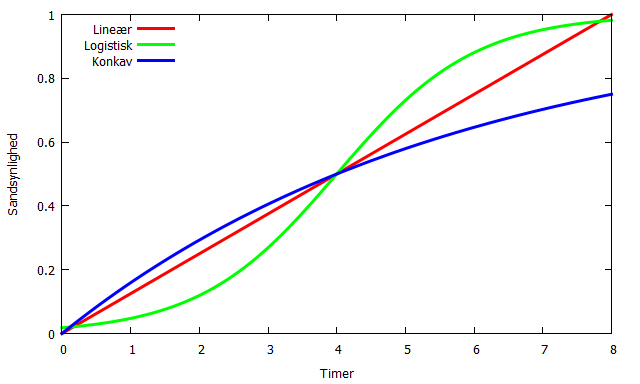
\includegraphics[scale=0.33]{graf-funktionseksempler}
	\caption{Tre funktioner til estimering af sandsynlighed for søvn}\label{fig:trefunc}
\end{figure}

\cref{fig:trefunc} viser tre forslag til en sådan funktion.
Disse er den røde lineære funktion, den blå konkave funktion og den grønne logistiske funktion \citep{wiki:LogisticFunction}.
Alle tre funktioner har til fælles at de er voksende, hvilket passer med vores antagelse af jo længere der har været stilstand jo større sandsynlighed er der for at man sover.
Den lineære funktion bygger på antagelsen, at sandsynligheden for at man sover er kongruent med stilstandslængden, hvilket vi ikke ønsker da vi så tillægger for stor vægt til korte stilstandsperioder. Imidlertid kan det godt være at den lineære og konkave funktion ville være bedre til at registrere korte søvnperioder midt om dagen.
Dette kræver videre arbejde men som en start benyttes den logistiske funktion, men kan nemt udskiftes.


Dn logistiske funktion beskriver hvordan at ved længere stilstandsperioder er der en forøget hældning i funktionen, indtil vi nærmer os lange stilstandsperioder hvor ekstra tid ikke giver en meget forøget sandsynlighed for søvn. 
Dette kan ses da den logistiske funktion vi har plottet går asymptotisk mod 1, svarende til 100\% sikkerhed for søvn.
I realiteten kan vi aldrig være 100\% sikker på søvn ved lang stilstand, da det kan være man har glemt sin telefon hjemme mens man er på tur over en weekend, men hvis forudsætningen for at systemet fungerer er at man har sin telefon i nærheden, regnes den logistiske funktion som et godt redskab til et søvnestimat.

Definitionen af den logistiske funktion er defineret som følger:
\begin{equation}
	f(t_{span}) = \frac{L}{1+e^{\,-k\cdot(t_{span} - t_{midtpunkt})}}
\end{equation} 
hvor,
\begin{itemize}
	\item[$L$] er kurvens maksimums værdi, hvilket for os eksempelvis kan være $1$ for 100\% sandsynlighed for at man sover.
	\item[$k$] er stejlheden for kurven.
	\item[$t_{span}$] Tidsperiode siden starten på stilstandsperioden målt i timer.
	\item[$t_{midtpunkt}$] Er det tidspunkt hvor kurven når $L/2$, hvilket i figurens tilfælde er hvornår kurven når $0.5$ det vil sige ved 4 timer.
\end{itemize}

Der kan argumenteres for en lavere værdi for $L$ så man maks kan blive 90\% sikker, men er noget der bør overvejes med mere træningsdata. 
Det kan også være en god idé at ændre på stejlheden for kurven, altså k, baseret på hvilken kilde af data man bruger som f.eks. accelerometer eller lyd.
Desuden skal $t_{midtpunkt}$ værdi på 4 timer betragtes som et første bud der passede fint med det observerede data, men kan justeres.

\subsection{Kombinering af modeller}\label{subsec:kombimodeller}
Det er tiltænkt at hver sensor kan have en tilknyttet søvnestimeringsmodel, hvilket i vores tilfælde er en søvnestimeringsmodel for accelerometret og en for amplituden.
Imidlertid kan det være en fordel at have en samlet model der kombinerer resultaterne fundet for de enkelte modeller.
En metode til dette er det vægtede gennemsnit og er et redskab vi har beskrevet i \cref{sec:redskaber}
Vores implementering af det vægtede gennemsnit afviger fra et normalt vægtet gennemsnit, idet at for de enkelte søvnestimeringsmoduler er der ikke blevet registreret data på samme tid eller i samme mængde.
På grund af dette tager modulet højde for hvis der er mangel på en estimering til en given tid for et af søvnestimeringsmodulerne.
Måden dette gøres er ved at tages den forrige værdi til estimeringen.
Man kan forestille sig en lynlås hvor der skiftes mellem takkerne fra hver del, på samme måde gøres med estimeringerne for hvert modul, for at illustrere dette bruges der et eksempel.

\newcommand{\nv}{Ingen estimering}

\begin{table}[h]
\centering
\begin{tabular}{|c|c|c|p{2.5cm}|}
\hline Tid & Sandsynlighed for model A & Sandsynlighed for model B & Resultat\\ 
\hline 02:30:00 & 	0.59    & \nv  	& $\text{Vægt}_A * 0.59 + \text{Vægt}_B * 0.29$\\ 
\hline 02:30:01 & 	\nv     & 0.29 	& $\text{Vægt}_A * 0.61 + \text{Vægt}_B * 0.29$\\ 
\hline 02:30:02 & 	0.61    & \nv 	& $\text{Vægt}_A * 0.61 + \text{Vægt}_B * 0.31$\\ 
\hline 02:30:03 & 	0.62    & \nv 	& $\text{Vægt}_A * 0.62 + \text{Vægt}_B * 0.31$\\ 
\hline 02:30:04 & 	\nv     & 0.31 	& ...\\
\hline 
\end{tabular} 
\als{Giv en række hvor begge har estimat}
\caption{Tabel der illustrerer hvordan kombineringen fungerer. $\text{Vægt}_A$ og $\text{Vægt}_B$ er de fastsatte vægte for de to modeller.}
\label{tab:combiModelsExample}
\end{table}

I \cref{tab:combiModelsExample} kan man se kombineringen af de to modeller.
Måden den kombinerer sandsynligheder på er ved at den starter med to gennemløbere, henholdsvis for A og B, som starter på det første element som ikke er tom. 
Så derfor i eksemplet vil A starte ved 02:30:00 med værdien $0.59$ og for B vil den starte ved 02:30:01 med værdien $0.29$. 
Disse to værdier kombineres for det bagerste element med vægtningerne for de to modeller, hvorefter flyttes den bagerste gennemløber, og en ny kombinering foretages.
Dette forsætter indtil der ikke er mere data tilbage i en af de to gennemløbere, hvorefter der ventes på ny data så begge gennemløbere igen har data at køre på.

\subsection{Aggregering}\label{subsec:soevnaggre}
Som demonstreret giver søvnestimeringsmetoden, der er vist som proof of concept, en estimering til en lang række tidspunkter.
Men for at give et ekstra redskab til at danne et overblik over disse estimeringer, kan der med fordel som proof of concept laves en aggregering af søvnestimeringsdata.

For at få et bedre indblik i formen af data der skal aggregeres gives et eksempel i \cref{tab:noaggsoevndata}.
\begin{table}[h]
	\centering
\begin{tabular}{|c|c|c|}
	\hline {\_}id & prob & time \\ 
	\hline 203754 & 0.050 & 2015-04-26 01:41:42.446 \\ 
	\hline 203755 & 0.050 & 2015-04-25 01:41:43.375 \\ 
	\hline ... & ... & ... \\ 
	\hline 218777 & 0.919 & 2015-04-26 05:52:36.204 \\ 
	\hline 218778 & 0.919 & 2015-04-26 05:52:37.203 \\ 
	\hline 218779 & 0.000 & 2015-04-26 05:52:38.163 \\ 
	\hline 
\end{tabular}
\caption{Eksempel på søvnestimeringsdata, der ikke er aggregeret.}\label{tab:noaggsoevndata}
\end{table}
Ved at se på data som i \cref{tab:noaggsoevndata} fremstår det hvordan at fra {\_}id 203754 til {\_}id 218778 er sandsynligheden for søvn, der ses i \textit{prob} kolonnen, monotont voksende.
Idéen derudfra er så at registrere sådanne monotoniforhold og aggregere data med hensyn til det.
Det vil sige at registrere intervaller hvor \textit{prob} er tilpas stor over en længere tidsperiode, samt er monotont voksende.

Det blev besluttet at forkaste intervaller kortere end 10 minutter og hvor sandsynligheden for søvn i slutningen af intervallet er under 10\%.
Dette kan være en fornuftig løsning under antagelse af at man er rolig når man sover, og har da også vist gode resultater med nogle tests af personer med en meget rolig søvn. 
Eksempelvis med det viste data i \cref{tab:noaggsoevndata} vil dette blive aggregeret til en række som set i \cref{tab:aggdat}.

\begin{table}[h]
	\centering
\begin{tabular}{|c|c|c|c|}
	\hline {\_}id & startdate & enddate & prob \\ 
	\hline 1 & 2015-04-26 01:41:42.446 &  2015-04-26 05:52:37.203 & 0.919 \\ 
	\hline 
\end{tabular} 
\caption{Aggregering af data fra \cref{tab:noaggsoevndata}.}\label{tab:aggdat}
\end{table}

Vi har dog også fundet tilfælde hvor en aggregering ikke er akkurat, eksempelvis ved snorken fejler denne aggregering da den er for naiv, yderligere diskussion om hvad man kan gøre i stedet for kan læses i \cref{section:snorken}.
Et alternativ kunne være at tage arealet af søvnestimeringsdata, og bruge arealet som estimat til hvor meget man har sovet per dag.
Dette har ulempen at det ikke vil oplyse om selve søvnperioderne men blot mængde af søvn per dag, derudover vil den stadig blive påvirket af snorken og andre støjfaktorer.
Vi hæfter os ved at denne aggregeringsmetode er ment som et proof of concept og med ekstra ressourcer kan det være fornuftigt at se på andre aggregeringsmetoder og inddrage fundne snorken estimeringer til at kunne aggregere søvndata på mere akkurat vis. Forslag til dette kan læses i \cref{section:snorken}.

\subsection{Visualisering}\label{sec:pocVis}
For at kunne vise brugeren af systemet hvordan deres søvn har været, skal der tilføjes nogle visningsmoduler.
Disse visningsmoduler skal kunne give et overblik over hvordan man har sovet den seneste nat, men også hvordan man har sovet det seneste stykke tid.

For at kunne udtrykke dette til brugeren er der først blevet lavet en graf der viser hvor sikker systemet er på at man har sovet over en periode.
Denne periode er sat til at være alt data der er på telefonen så brugeren har overblik over ændringer i grafen.
Disse ændringer kan derved indikere at der er sket en ændring i ens sindstilstand.
Til at sørge for at grafen kan bruges til både at se hvordan man har sovet over en længere periode samt over en kort periode, har man den mulighed at man kan zoome på grafen, og derved se præcis hvor sikker systemet er på man har sovet på et bestemt tidspunkt.
Der er også lavet en graf for hvor sikker systemet ved hjælp af kun acceleration er på at man sover, det samme gælder for lyd, se \cref{fig:visningsgrafer}.

\begin{figure}[h]
	\centering
	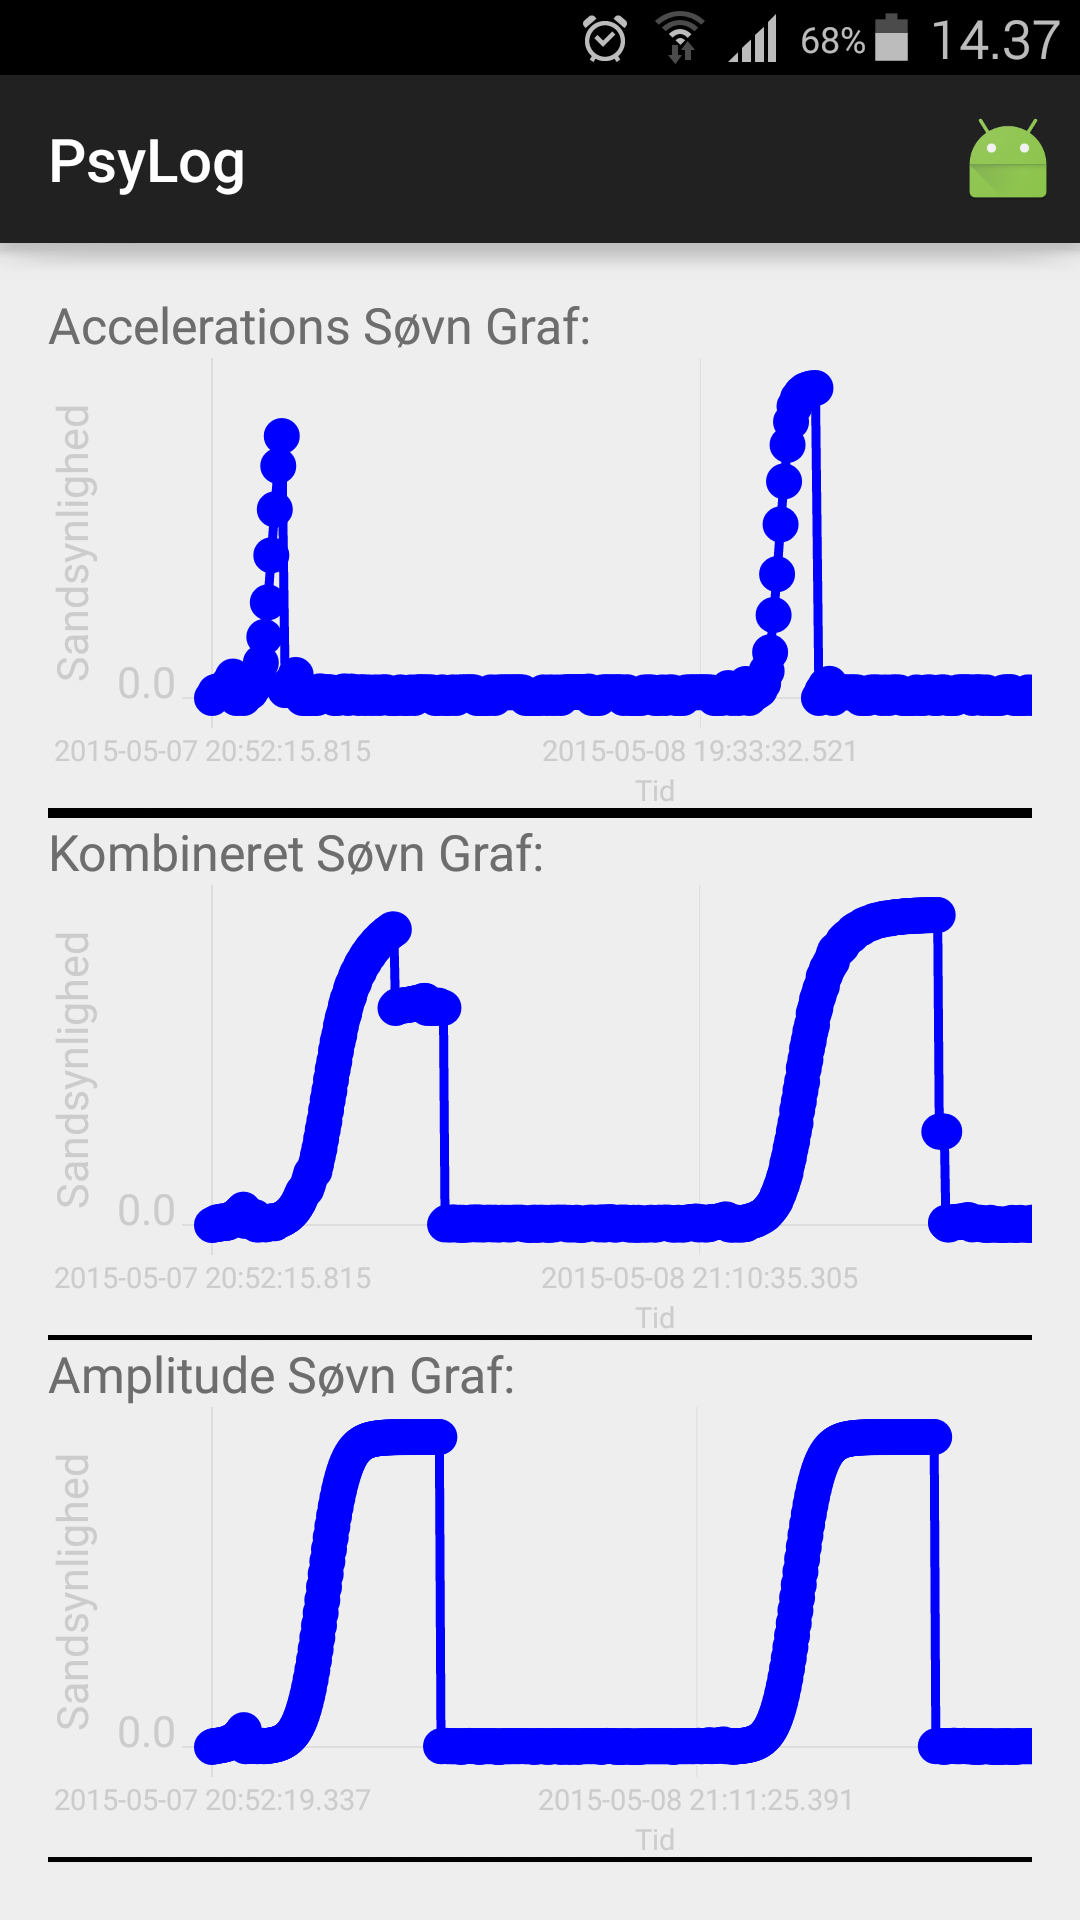
\includegraphics[scale=0.1]{visningsgrafer}
	\caption{Tre funktioner til estimering af sandsynlighed for søvn}\label{fig:visningsgrafer}
\end{figure}

Grafer er dog ikke altid lige nemme at forstå, derfor er der blevet lavet en tabel der viser hvor sikker systemet er på at man har sovet over en periode.
Denne tabel minder om den der blev vist i \cref{tab:aggdat}, dog uden $\_id$ kolonnen.
Tabellen giver et nemt overblik for brugeren om hvornår man har sovet, samt hvor sikker systemet er på at man har sovet.
Dog er det ikke så nemt for brugeren at se ens adfærdsændring i en sådan tabel, da det kræver at man kigger på meget data på en gang.
Som alternativ kan der ses på et 'early warning modul', og er diskuteret i \cref{chap:bigdisc}.
% Giv eksempel på ikke aggregeret data.
% Forklar forslag/løsning til aggregering af data.
% Vis resultat derfor
% Diskuter problemer? (e.g. snorken) evt. referer til snorken diskussion